\documentclass{article}
\usepackage{longtable}
\usepackage{graphicx}
\usepackage{booktabs}% http://ctan.org/pkg/booktabs
\newcommand{\tabitem}{~~\llap{\textbullet}~~}
\usepackage{array}
\usepackage[style=numeric,backend=bibtex]{biblatex}
\usepackage{caption}
\usepackage{amsmath}

\bibliography{Parken}

\begin{document}

\title{SoNah Parken Analytics}
%subtitle
\author{Andrei Ionita}

\maketitle

\section{Einf\"uhrung}
SoNah ist ein Parkplatz Informationssystem, das Fahrern dabei hilft, einen Parkplatz schnell und unkompliziert in der Stadt zu finden. SoNah verf\"ugt \"uber eine wachsende Menge an Parksensoren, die in St/"adten an diversen Partner-Parkpl\"atze oder an E-Ladestadtionen montiert sind. Die Sensoren heben anonymisierte Parkinformationen ab, die dann so auswertet werden, dass zun\"achst den Ist- Zustand des Parkraums abbilden. Seine technische St\"arke liegt darin, Anfragen zu frei werdenden Parkpl\"atze anhand historischen Daten und der aktuellen Lage zu beantworten.

\vspace{2mm}
Der typische Anwendungsfall ist:

\vspace{2mm}
\textit{Mirko f\"ahrt von A nach B. Er ist nicht nur daran interessiert, schnell und sicher, geleitet von seinem Navi in B anzukommen, sondern auch in B unkompliziert zu parken. Mirko pr\"uft den Zustand der verf\"ugbaren Pl\"atze in B bereits bei der Abfahrt, jedoch abh\"angig von der Reisedauer kann sich die Parksituation um $180^\circ$ ver\"andern. Deshalb braucht Mirko ein zuverl\"assiges und pfiffiges System, das ihn auf einen freien Parkplatz hinweist. Mirko probiert SoNah und stellt fest, dass SoNah diese Anforderungen v\"ollig erf\"ullt.}

\section{Ziel der Masterarbeit}
Im Rahmen dieser Masterarbeit wird ein System entwickelt, dass Vorhersagen \"uber die Parkplatzsituation an verschiedenen Orten und Zeitpunkten liefern kann. Die Parkdaten (m\"oglicherweise Parksensoren, Partnerdatenquellen, historische Daten o.a.) werden so auswertet, dass Anfragen auf freie Parkpl\"atze mit Bezug auf aktuellen und k\"unftigen Zustand richtig und m\"oglichst effizient beantwortet werden. Das System sollte instande sein, Anfragen wie in der Tabelle~\ref{tabelle} zu beantworten.

{\small
\begin{longtable}{| c | >{\raggedright\arraybackslash}p{9cm} |}%[!ht]
 %\centering
  %\begin{tabular}{ | c | >{\raggedright\arraybackslash}p{9cm} | }
    \hline
     & \multicolumn{1}{c|}{\textbf{Anfragen}} \\ \hline
    \textbf{Parksensor} & \tabitem Stellt fest, ob ein bestimmter Parkplatz zurzeit frei ist \\ 
     		   & \tabitem Stellt fest, wie viele Pl\"atze in einem bestimmten Parkraum zurzeit frei sind \\ \hline 
    \textbf{Analytics} & \tabitem Berechnet die Wahrscheinlichkeiten, dass ein Parkraum in der Zukunft mindestens einen Parkplatz frei hat \\
    			& \tabitem Weist einen Parkplatz im Parkraum einem Auto zu, sodass die restlichen freien Parkpl\"atze gleichm\"a\ss{}ig verteilt bleiben \\ \hline
    \textbf{User} & \tabitem Findet heraus, ob bei der Ankunft mindestens ein Parkplatz im Parkraum frei wird \\ 
    	& \tabitem Findet heraus, wie viele Parkpl\"atze im Parkraum an einem bestimmten Tag frei sind \\
    	& \tabitem Falls der Parkraum aktuell mindestens einen Parkplatz verf\"ugbar hat, weist dem User einen Parkplatz zu \\ \hline
  %\end{tabular}
	\caption{Funktionalit\"at auf Ebenen}
 	\label{tabelle}
\end{longtable}}


\section{Architektur}
Die Analytics Komponente wird mit den anderen Teilen des Systems Daten austauschen (siehe Figur~\ref{fig:architektur}). Die User-Interface stellt ihnen Fragen bzgl. der Verf\"ugbarkeit der Parkpl\"atze, die sie synchron beantwortet bekommt. Daten von Sensoren und andere Datenquellen (historische Stadtdaten, Partnerdaten, etc.) stehen Analytics immer zur Verf\"ugung und dienen zum asynchronen Modellbildung.

\vspace{4mm}
\begin{figure}[!ht]
    \centering
    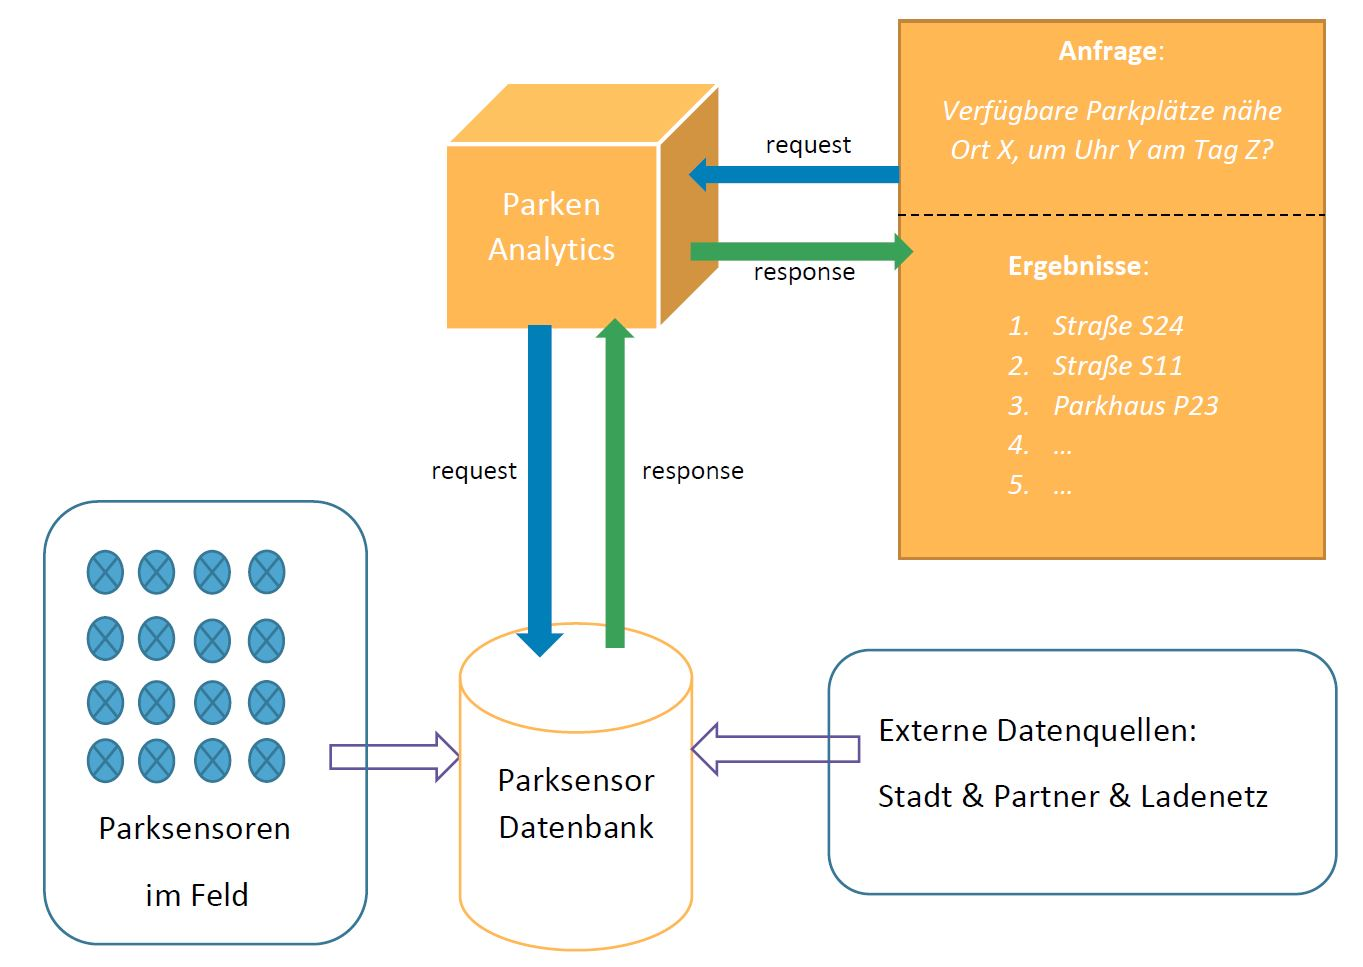
\includegraphics[width=4.5in]{Architektur}
    \caption{Systemkomponente und deren Zusammenspiel}
    \label{fig:architektur}
\end{figure}

\section{Sto\ss{}zeiten}
Neben Antworten auf einzelne Anfragen kommt SoNah den Fahrern mit langfristigen Prognosen \"uber gesamte Parkbereiche entgegen. Unter Ber\"ucksichtigung von Wochentag, Tageszeit und weitere Einfl\"ussen wird das System in der Lage sein, Statistiken \"uber die Zahl der freien Parkpl\"atze zu erstellen (siehe Figur~\ref{stosszeiten}).

\begin{figure}[!ht]
    \centering
    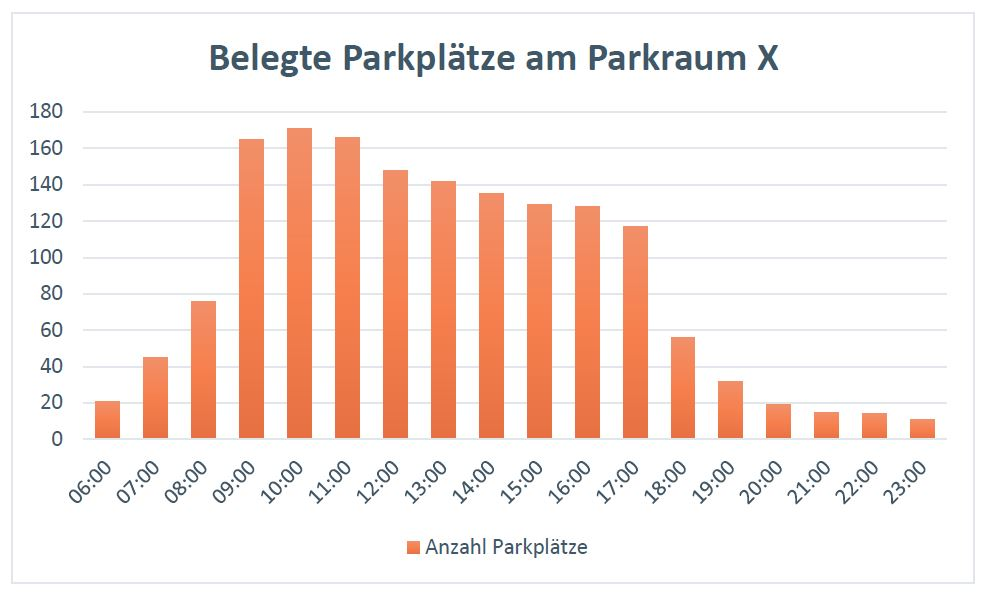
\includegraphics[width=4.0in]{Stosszeiten}
    \caption{Sto\ss{}zeiten-Diagramm f\"ur einen Parkraum}
    \label{stosszeiten}
\end{figure}


\section{Voraussichtliches Konzept}
\subsection{Theorie}
Die zeitliche Entwicklung der wahrscheinlichsten Anzahl freier Parkpl\"atze lassen sich als Markov Ketten modellieren\cite{Caliskan2007}. Die Frequenz der Einfahrten $\lambda$ und die Parkdauer $\mu^{-1}$ gen\"ugen erst einmal, um das Modell zu bestimmen. Die Anzahl freie Parkpl\"atze in $t$ Zeiteinheiten, die von i auf j Pl\"atze ver\"andert, wird als $p_{ij}(t)$ bezeichnet.

\vspace{2mm}
Um diese Werte herauszufinden, sind zuerst die \"Ubergangswerte $q$ zu berechnen:

$$q_{ij} = \lim_{t\to0} \frac{p_{ij}(t)}{t}$$

\vspace{2mm}
Die Gesamtwahrscheinlichkeit ergibt sich nach folgendem Zusammenhang:
$$q_{ii} = - \sum_{j\neq i} q_{ij}$$

\vspace{2mm}
Die gesamte $q$ Matrix wird wie folgt aussehen:

\vspace{2mm}
q = 
$
\begin{pmatrix}
-\lambda & \lambda & \dots &  &  &  \\
\mu & -(\lambda + \mu) & \lambda & \dots &  &  \\
\dots & 2\mu & -(\lambda + 2\mu) & \lambda & \dots & \\
 & \dots & \dots & \dots & \dots & \dots \\
 &  & \dots & (m-1)\mu & -(\lambda + (m-1)\mu) & \lambda \\
 &  &  & \dots & m\mu & -m\mu
\end{pmatrix}
$

\vspace{6mm}
Die resultierende Matrix $q$ ist $(m+1) \times (m+1)$ gro\ss{}, wobei $m$ die Anzahl der Parkpl\"atze am jeweiligen Parkraum ist. $q_{s_1s_2}$ bezeichnet die Wahrscheinlichkeit dass sich die Anzahl gleich von $s_1$ freien Parkpl\"atzen auf $s_2$ freie Parkpl\"atze ver\"andert.

Weitere Ans\"atze werden w\"ahrend der Literaturrecherche-Phase identifiziert und im Rahmen der angegebenen Bedingungen wird der passende Ansatz ausf\"uhrlich beschrieben und angewendet.

\subsection{Praxis}
Das Modul wird voraussichtlich im Python oder Java implementiert. Es bleibt offen, ob es entweder als einfache Backend Bibliothek und ein separates UI oder als MVC Anwendung (e.g. in Django) umgesetzt wird.

\subsection{Evaluation}
Anhand der angesammelten Parksensordaten werden erste Prognosen geliefert. Beim Testen wird nicht die gesamte Datenbestand verwendet, damit die Ergebnisse mit den sp\"ater abgespeicherten Parkdaten verglichen werden k\"onnen, e.g. die fr\"uheren 70\% der Daten f\"ur das Modellbildung, die sp\"ateren 30\% f\"ur das Testen.

\vspace{2mm}
Alternativ, bei unzureichenden Sensordaten l\"asst sich das Testen durch unabh\"angiges Simulieren einer kontinuierlichen Parksituation durchf\"uhren.

\section{Zeitplan (vorl\"aufig)}

\begin{table}[!ht]
 \centering
  \begin{tabular}{|c|l|}
  \hline
  	1. - 2. Woche & Proposal erstellen / Forschungsfrage formulieren \\ \hline
  	3. - 6. Woche & Literaturrecherche \\ \hline
  	6. - 9. Woche & Konzept aufbereiten \\ \hline
  	10. - 17. Woche & Implementierung \\ \hline
  	18. - 21. Woche & Evaluation \\ \hline
  	22. - 25.  Woche & Abschlie\ss{}en \\ \hline
  	& \\ \hline
  \end{tabular}
\end{table}

\nocite{*}

\printbibliography

\end{document}